%; whizzy chapter
% -initex iniptex -latex platex -format platex -bibtex jbibtex -fmt fmt
% $B0J>e(B whizzytex $B$r;HMQ$9$k>l9g$N@_Dj!#(B

%     Tokyo Debian Meeting resources
%     Copyright (C) 2011 Junichi Uekawa
%     Copyright (C) 2011 Nobuhiro Iwamatsu

%     This program is free software; you can redistribute it and/or modify
%     it under the terms of the GNU General Public License as published by
%     the Free Software Foundation; either version 2 of the License, or
%     (at your option) any later version.

%     This program is distributed in the hope that it will be useful,
%     but WITHOUT ANY WARRANTY; without even the implied warranty of
%     MERCHANTABILITY or FITNESS FOR A PARTICULAR PURPOSE.  See the
%     GNU General Public License for more details.

%     You should have received a copy of the GNU General Public License
%     along with this program; if not, write to the Free Software
%     Foundation, Inc., 51 Franklin St, Fifth Floor, Boston, MA  02110-1301 USA

%  preview (shell-command (concat "evince " (replace-regexp-in-string "tex$" "pdf"(buffer-file-name)) "&"))
% $B2hA|%U%!%$%k$r=hM}$9$k$?$a$K$O(Bebb$B$rMxMQ$7$F(Bboundingbox$B$r:n@.!#(B
%(shell-command "cd image201109; ebb *.png")

%%$B$3$3$+$i%X%C%@3+;O!#(B

\documentclass[mingoth,a4paper]{jsarticle}
\usepackage{monthlyreport}

% $BF|IU$rDj5A$9$k!"Kh7nJQ$o$j$^$9!#(B
\newcommand{\debmtgyear}{2011}
\newcommand{\debmtgmonth}{10}
\newcommand{\debmtgdate}{22}
% (+ (* (- 2011 2005) 12) 9 -1) started from zero
\newcommand{\debmtgnumber}{81}

\begin{document}

\begin{titlepage}
\thispagestyle{empty}
% $B%?%$%H%k%Z!<%8(B:$BJT=8I,MW$JItJ,$O:G=i$N%^%/%m$KHt$P$9$3$H(B

\vspace*{-2cm}
$BBh(B\debmtgnumber{}$B2s(B $BEl5~%(%j%"(B Debian $BJY6/2q;qNA(B\\
\hspace*{-2cm}
\includegraphics[width=210mm]{image201003/debsen.eps}\\
\hfill{}\debmtgyear{}$BG/(B\debmtgmonth{}$B7n(B\debmtgdate{}$BF|(B

% $B$3$3$O%"%C%W%G!<%H$9$k$3$H(B
\rotatebox{10}{\fontsize{32}{32} {\gt $BFC=8(B1: Haskell$B$H(BDebian$B$N?I$/$F4E$$4X78(B}}

\rotatebox{10}{\fontsize{32}{32} {\gt $BFC=8(B2: YYYY}}

\vspace*{-2cm}
\hfill{}
\includegraphics[height=6cm]{image200502/openlogo-nd.eps}
\end{titlepage}

\dancersection{Introduction}{$B>e@n(B $B=c0l(B}

\begin{multicols}{2}
 

 $B:#7n$N(BDebian$BJY6/2q$X$h$&$3$=!#$3$l$+$i(BDebian$B$N@$3&$K$"$7$rF'$_F~$l$k$H(B
 $B$$$&J}$b!"$9$G$K$I$C$W$j$H$D$+$C$F$$$k$H$$$&J}$b!"7n$K0l2s(BDebian$B$K$D$$(B
 $B$F8l$j$^$;$s$+!)(B

 Debian$BJY6/2q$NL\E*$O2<5-$G$9!#(B

 \begin{itemize}
 \item \underline{Debian Developer} ($B3+H/<T(B)$B$N0i@.!#(B
 \item $BF|K\8l$G$N!V(B\underline{$B3+H/$K4X$9$k>pJs(B}$B!W$r@0M}$7$F$^$H$a!"%"%C%W%G!<%H$9$k!#(B
 \item \underline{$B>l(B}$B$NDs6!!#(B
 \begin{itemize}
  \item $BIaCJ$P$i$P$i$J>l=j$K$$$k?M!9$,(B face-to-face $B$G=P2q$($k>l$rDs6!(B
	$B$9$k!#(B
  \item Debian $B$N$?$a$K$J$k$3$H$r8l$k>l$rDs6!$9$k!#(B
  \item Debian$B$K$D$$$F8l$k>l$rDs6!$9$k!#(B
 \end{itemize}
 \end{itemize}		

 Debian$B$NJY6/2q$H$$$&$3$H$G5f6KE*$K$O;22C<TA40w$,(BDebian Package$B$r$,$j$,$j(B
 $B$H:n$k%9!<%Q!<%O%C%+!<$K$J$C$?;Q$rLQA[$7$F$$$^$9!#>pJs$N6&M-!&3hMQ$rDL$7(B
 $B$F(B Debian$B$N:#8e$NG=F0E*$JE83+$X$NEZBf$H$7$F!"!V>l!W$H$7$F$N6u4V$rDs6!$9(B
 $B$k$N$,L\E*$G$9!#(B

\end{multicols}

\newpage

\begin{minipage}[b]{0.2\hsize}
 \definecolor{titleback}{gray}{0.9}
 \colorbox{titleback}{\rotatebox{90}{\fontsize{80}{80} {\gt $B%G%S%"%sJY6/2q(B} }}
\end{minipage}
\begin{minipage}[b]{0.8\hsize}
\hrule
\vspace{2mm}
\hrule
\begin{multicols}{2}
\tableofcontents
\end{multicols}
\vspace{2mm}
\hrule
\end{minipage}

\dancersection{$B;vA02]Bj(B}{$BA0ED(B $B9LJ?(B}

$B:#2s$N;vA02]Bj$O0J2<$G$9(B:
\begin{enumerate}
 \item $B:#!"%3%s%T%e!<%?$r;H$C$F$"$J$?$,$d$j$?$$$3$H!"$d$C$F$$$k$3$H$O$J$s$G$9$+!)$=$l$O(BDebian($B$^$?$O(BLinux)$B$G$G$-$^$9$+!)(BDebian($B$^$?$O(BLinux)$B$r;H$C$F$J$1$l$P$=$NM}M3$r65$($F2<$5$$!#(B
\end{enumerate}
$B$3$N2]Bj$KBP$7$FDs=P$$$?$@$$$?FbMF$O0J2<$G$9!#(B
\begin{multicols}{2}
{\small
% \begin{prework}{ ����(yy\_y\_ja\_jp) }
���ޤ���������ǤϤʤ��Ǥ���... �긵�Υ�åץȥåפǤ� /boot �ˤ� ext2
 ����¾�ˤ� ext3���Ƕ�ȤäƤ���ǥ����ȥåפǤ� /boot �ˤ� ext3 ����¾
 �ˤ� LVM ��� ext4 ��ȤäƤ��ޤ���
\end{prework}

\begin{prework}{ �����ϥ� }
�ǥե���Ȥ�ext3����
�����ǥե���ȤΤޤޡ�
(NTFS���VM���᡼�����ext3�⤢�뤱��)
\end{prework}

\begin{prework}{ yos.takahashi }
ext3/4���˻ȤäƤޤ���ext3�Υǡ�������١����ˤĤ�������Linux2011ǯ1���˼�ɮ���ޤ�����
\end{prework}

\begin{prework}{ MATOHARA }
����inode �ϳ���������Ƥ���inode ��ưŪ�˳�����Ƥ���XFS �����򤹤뤳
 �Ȥ�¿���Ǥ���NILFS �Ͼ�����Ƥߤ��ΤǤ�����mount ���˰ʲ��Τ褦�ʥ��
 ���������ФƤޤ��ݤ��ʤȻפ��ޤ�����
\begin{commandline}
$ sudo mount /dev/sdb1 /mnt
mount.nilfs2: WARNING! - The NILFS on-disk format may change at any time.
mount.nilfs2: WARNING! - Do not place critical data on a NILFS filesystem. 
\end{commandline}
����¾NotePC �Ǥ�dm-crypt �ξ�˥ե����륷���ƥ���֤��ưŹ沽�����ꡢ
 eCryptfs �ǰŹ沽�����ꤷ�Ƥ��ޤ����񤭹��߻���CPU �򤫤ʤ���񤷤ޤ��ġ�
\end{prework}

\begin{prework}{ ��ޤ� }
��ext2-$>$reiserfs-$>$jfs-$>$xfs-$>$reiserfs-$>$ext3�ȻȤäƤ��ޤ�����

����:
\begin{itemize}
 \item reiserfs: ���ե������¿���ե�����Υ������������ӥ��Ӥ��Ƥ��ɤ���
       �����������դȤ����ⵤ�������θ�μ�žȬ�ݥ����ɤˡ�����
 \item jfs: ����v1.0��̾��ä�IBM���ꥨ�ʥ��������ˤ�xfs��ƨ��
 \item xfs: fsck==true�˴�ư����������ǯ�Ȥä���ΤΥޥ�����Ĵ����0byte
       �ե��������������Ѥ���줺ƨ����
\end{itemize}
������reiser4��Ķ���Ԥ��뤦���ˤ��줬�����ʤäơ����ext3�˸��경��htree�����ä������⤦Ŵ�Ĥʤ鲿�Ǥ⤤���Ǥ��������Ȥ����Ĥ�nilfs�ʤɤ˼��Ф��Ƥ��ޤ���ext3�������noatime���٤Ǥ����������aufs���碌�Ƽ�ʬ���Ȥ��Ȥ� *strap �Ķ��򥯥����˥󥰤��Ƥ��ޤ����¸����ƥ��Ȥ������Ǥ�����Ǥ���USB�����ư�Ǥ�ͭ�ѡ�

���LVM�ǤϤʤ�MD��Ȥäƾ�Ĺ���ܥХå����åפ򤷤Ƥ��ޤ���
 MD(sda,sdb,sdc)�ǹ��ۤ����̾��MD(����)�Dz�ư���Хå����åפλ���
 attach/detach�򤹤롣�֥��å���٥�ʤΤǥꥫ�Х��FSǤ���Ǥ��������̤�
 �������¾����ˡ���ʤ�������
\end{prework}

\begin{prework}{ henrich }
�ȤäƤ���֤�NTFS��Ĺ���󤸤�ʤ��Ǥ����͡����졣
�����Ρ����Ѥο������ǥ�������ext4�ǥե����ޥåȤ��ޤ����������㤤��Ƚ��ʤ��Ȥ����������Ƥ��ޤ���
\end{prework}

\begin{prework}{ emasaka }
�Ĥ뤷��FS��ȤäƤޤ�
\end{prework}

\begin{prework}{ �ܾ� }
ext3����Ѥ��Ƥ��ޤ����ä��Ѥ�ä����ȤϤ��Ƥ��ޤ���
FS����ʤ��Ǥ������Ƕ�Lenny��2TB��HDD��Ȥä���parted�äƤλȤ��ƶä��ޤ�����
\end{prework}

\begin{prework}{ ����@������ }
���������Ū�˳��Ѥ��Ƥ���ե����륷���ƥ��ReiserFS�Ǥ���
�Ż��ǻȤäƤ�Ķ���ext3�Ǥ�����ext3���Ÿ������ǥ��㡼�ʥ뤬
����Ʋ��Ǥ������ηи��ʸŤ������ͥ�Ǥ���...�ˤ����ꡢ
���ޤ꿮�Ѥ��Ƥ��ޤ���
�����ReiserFS�Ķ��ǤϤ���ޤǤνꤤ���ʤ��Ÿ����ڤä��ꡢ
�Ƥ�HDD�����줫�����ꤷ�Ƥ��ﳲ����ä��и���̵���Τǡ�
��³Ū�˻ȤäƤ��ޤ���
��ǯ����ReiserFS�Υᥤ��ȯ��(Hans Reiser)�����ᤵ��Ƥ��ޤ������ƥʥ󥹤��ۤ��Ƥ��ޤ�����
�����������θ��ReiserFS��¾�γ�ȯ�Ԥˤ���³�����ݼ餵��Ƥ���Τǡ��¿����ޤ�����
\end{prework}

\begin{prework}{ nozzy123nozzy }
\begin{enumerate}
 \item LVM�ˤĤ��Ƥϡ�CentOS5.5��Ƴ�������Τ��Τޤޤ����Ѥ��Ƥޤ�����
       ���������ƥब��äƤ���Volume̾�ϥǥե���Ȥ�����ȡʼºݤˤ�
       kickstart�ˤơˤ��ѹ����ƻȤäƤޤ����ʾ㳲���Υ���١����˺��뤿
       ���
\item ext3�ˤĤ��Ƥϡ�debian-sid�����Τޤ޻��ꤷ�Ƥ����Τ򤽤Τޤ޻Ȥ�
      �Ƥ����ꤷ�ޤ���relatime, noatime ���餤�Ͼ����ɲä��Ƥߤ����ʡ���
      �ϻפäƤޤ���
\end{enumerate}
\end{prework}

\begin{prework}{ �ޤ��������ؤ� }
\begin{itemize}
 \item Debian�Ǥ��ä˶Ťä����Ȥ�����ext3��ȤäƤޤ������ۥޥ����qcow2
       ���᡼���ǥ��������ѻ��ʳ��ϡ�LVM�ϻȤäƤޤ���
 \item �����ǰ����ü�ʤΤϡ��������DHCP�������Ѥ�Armadillo-J�ǻȤäƤ�
       ��JFFS�Ǥ����ǥե���ȤΥե����०�����Ǥϥ�֡��Ȥ�����������
       �ƽ��������Ƥ��ޤ��Τǡ�RAM�ΰ�˽񤭤��ߡ��Ÿ��ڤäƤ�ä��ʤ�
       ���������Ǥ���Debian��udhcp�Υ������ѥå���������ӥ�ɤ��ƻȤäƤޤ���
       \footnote{\url{http://d.hatena.ne.jp/mkouhei/20080601/1212330630}}
 \item ��Debian���ߤǡ���ʬ����ǰ��֥ۥåȤʤΤ�palm webOS�Ǥ��������Ubuntu��
       �������ޥ���������Τ餷���ΤǤ�����/etc/mtab�򸫤��35�Ԥ⤢�ꡢ
       ���ʤ����֤ʹ����Ǥ��͡�
\end{itemize}
\end{prework}
}
\end{multicols}

\dancersection{$B:G6a$N(BDebian$B4XO"$N%_!<%F%#%s%0Js9p(B}{$BA0ED(B $B9LJ?(B}
\subsection{$BEl5~%(%j%"(BDebian$BJY6/2q(B80$B2sL\Js9p(B}

$B0KF&$N29@t$K$$$C$F(BDebian$B$N3+H/$r$7$F$$$^$7$?!#;22C<T$O#8L>$G$7$?!#(B

% (query-replace-regexp "<.*?>" "")
% (query-replace-regexp "^[	 ]\+" "")



\dancersection{Debian Trivia Quiz}{$BA0ED(B $B9LJ?(B}

$B$H$3$m$G!"$_$J$5$s(B Debian $B4XO"$NOCBj$K$*$$$D$$$F$$$^$9$+!)(BDebian$B4XO"$NOC(B
$BBj$O%a!<%j%s%0%j%9%H$r$h$s$G$$$k$HDI@W$G$-$^$9!#$?$@$h$s$G$$$k$@$1$G$O$O(B
$B$j$"$$$,$J$$$N$G!"M}2rEY$N%F%9%H$r$7$^$9!#FC$K0l?M$@$1$G$O0UL#$,$o$+$i$J(B
$B$$$H$3$m$b$"$k$+$bCN$l$^$;$s!#$_$s$J$G0l=o$KFI$s$G$_$^$7$g$&!#(B

$B:#2s$N=PBjHO0O$O(B\url{debian-devel-announce@lists.deban.org} $B$d(B \url{debian-devel@lists.deban.org}$B$KEj9F$5$l$?(B
$BFbMF$H(BDebian Project News$B$+$i$G$9!#(B

\begin{multicols}{2}
% %; whizzy-master ../debianmeetingresume201101.tex
% 以上の設定をしているため、このファイルで M-x whizzytex すると、whizzytexが利用できます。
%
% ちなみに、クイズは別ブランチで作成し、のちにマージします。逆にマージし
% ないようにしましょう。
% (shell-command "git checkout quiz-prepare")

\santaku
{Debian温泉2011の1日目はいつでしょうか?}
{9/17}
{9/18}
{9/19}
{A}
{さっきの話を聞いていればわかって当然ですね}

\santaku
{8月にDebianは誕生日を迎えました。何周年でしたでしょうか?}
{17}
{18}
{19}
{B}
{今年もお祝いしましたよね}

\santaku
{最新のDebian Newsはいつ発行されたでしょうか?}
{9/17}
{9/18}
{9/19}
{C}
{購読していれば知っていて当然ですね}

\santaku
{10/17の''delegation for the DSA team''で代表団に任命されなかったのは誰でしょう?}
{Faidon Liambotis}
{Luca Filipozzi}
{Nobuhiro Iwamatsu}
{C}
{他に任命されたのは、の全部で合計名です。}

\santaku
{Wheezyフリーズの予定はいつでしょう?}
{2012年4月}
{2012年6月}
{2012年8月}
{B}
{あと6ヶ月ですよ!}

\santaku
{1.16.1がリリースされたdpkgに該当するのはどれ?}
{\texttt{dpkg-buildpackage}コマンドでは \texttt{CFLAGS, CXXFLAGS, LDFLAGS, CPPFLAGS, FFLAGS}の\texttt{export}が必須になった}
{\texttt{dpkg-deb}コマンドに\texttt{--verbose}オプションが追加された}
{Multi-Archフィールドがサポートされた}
{B}
{\texttt{dpkg-buildpackage}ではこれらのオプションが不要になりました。Multi-Archは1.16.2からサポートされる予定です。\texttt{dpkg-deb -x/--extract -v/--verbose}で\texttt{dpkg-deb -X/--xextract}と同じ動きをするようになりました。}

\end{multicols}

%-------------------------------------------------------------------------------
\dancersection{Haskell$B$H(BDebian$B$N?I$/$F4E$$4X78(B}{$B2,It5f(B}
%-------------------------------------------------------------------------------
\index{haskell}

\subsection{Haskell$B$H$$$&%W%m%0%i%_%s%08@8l(B}

Haskell \footnote{\url{http://haskell.org/}}
$B$H$$$&%W%m%0%i%_%s%08@8l$r$4B8CN$G$7$g$&$+!#(B
Haskell$B$O4X?t7?8@8l$N0l<o$G0J2<$N$h$&$JFCD'$,$"$j$^$9!#(B
($B0J2<$N0U8+$O(BHaskell$B=i?4<T$G$"$kI.<T$NJP8+$d4V0c$$$rB?NL$K4^$s$G$$$^$9(B)

\begin{itemize}
\item $B@EE*7?IU$1(B

$B0EL[$N7?JQ49$H$+$=$s$J$3$H$O5/$-$^$;$s!#(B
$B$^$?B?$/$N%(%i!<$r%3%s%Q%$%k;~$K8!=P$9$k$3$H$,$G$-$^$9!#(B
Haskell$B$G%W%m%0%i%_%s%0$r$7$F$$$k$H;kLn3Q$,69$/$J$k5$J,$K$J$k$H;W$$$^$9!#(B
$B7?$G<i$i$l$k$3$H$K$h$C$F!V9MN8$KF~$l$F$*$/$Y$-A0Ds!W$N%3!<%IHO0O$,>.$5$/$J$j!"(B
$B$=$7$F%$%s%?!<%U%'%$%9$KMQ$$$F$$$k7?$K$D$$$F!VK\Ev$K$3$l$,$U$5$o$7$$$N$+!)!W(B
$B$H9M$($k$3$H$K$J$j$^$9!#(B
$B$b$C$H4JC1$K8@$&$H!V7?$K$h$k@_7W!W$r(BHaskell$B$G$O9T$J$$$^$9!#(B

\item $B7??dO@(B

$B7?$r$9$Y$F=q$/I,MW$,$J$$$H$$$&MxE@$b$"$j$^$9$,!"(B
$B7??dO@$,$J$$$He:No$KI=8=$G$-$J$$$3$H$b$"$j$^$9!#(B
$B8D?ME*$K$O!"4X?t<+BN$K$O7?$r=q$$$F!"4X?t$NFbIt$G$N7?$O>JN,$9$k$3$H$,9T57$,(B
$BNI$$$H;W$$$^$9!#(B

\item $B%Q%?!<%s%^%C%A(B

if$B$d(Bcase$BJ8$G>l9gJ,$1$r5-=R$9$k$h$j$b$O$k$+$K=@Fp$J>l9gJ,$1$,$G$-$^$9!#(B
$B%"%k%4%j%:%`$N5-=R$H$O$"$k<o>l9gJ,$1$N7+$jJV$7$H$b8@$($k$N$G!"(B
$B$3$N>l9gJ,$1$r7?$G5-=R$G$-$k$H!"$o$+$j$d$9$/4J7i$K$J$j$^$9!#(B

\item $BCY1dI>2A(B

$B=t?O$N7u$G$9$,!"L58B%j%9%H$r:n$l$?$j!"GK2uE*$J%G!<%?9=B$$rMQ$$$J$/$F$b7W;;NL$r(B
$B>/$J$/$9$k$3$H$,$G$-$^$9!#(B
$B@53J@-%U%i%0$r;H$&$3$H$GCY1dI>2A$rItJ,$4$H$KM^@)$9$k$3$H$b$G$-$^$9!#(B

\item $B%3%s%Q%$%k$7$F<B9T(B

$B%m!<%+%k$G%3%s%Q%$%k$9$l$P!"G[I[@h$K$O(BHaskell$B$,%$%s%9%H!<%k$5$l$F$$$J$/$F$b(B
OK$B$G$9!#MW$OC1$J$k<B9T%P%$%J%j$K$J$j$^$9!#(B
$B$^$?(Brunhaskell$B%3%^%s%I$G%3%s%Q%$%k$;$:$K<B9T$9$k$3$H$b$G$-$^$9!#(B

\item $BFI$_$d$9$/!"=q$-$d$9$$J8K!(B

$BK\Ev$G$9(B!
$B$b$77?$r;H$C$F$bITB-$J%1!<%9$G$O(BTemplate Haskell
\footnote{\url{http://www.kotha.net/ghcguide_ja/latest/template-haskell.html}}
$B$r;H$($P%3%s%Q%$%k;~$K%a%?%W%m%0%i%_%s%0$r$9$k$3$H$b$G$-$^$9!#(B
$B8D?ME*$K$O8+$?L\$,$"$^$j$K$+$o$j$9$.$F$7$^$&$N$G!"<Y0-$J$N$G$O$J$$$+$H(B
$B;W$C$F$$$^$9$,!#!#!#$^$!;H$$$I$3$m$K5$$r$D$1$^$7$g$&!#(B

\end{itemize}

$B$I$&$G$7$g$&!#$o$/$o$/$7$^$9$h$M(B!
$B$5$C$=$/;H$C$F$_$^$7$g$&!#$J$!$K(BDebian$B$J$i4JC1$G$9!#(B
haskell-platform$B%Q%C%1!<%8$r%$%s%9%H!<%k$9$l$P(BHaskell$B%3%s%Q%$%i$G$"$k(Bghc$B$H(B
$B$=$N4pK\%i%$%V%i%j72$,;H$($k$h$&$K$J$j$^$9!#(B
Ruby$B$N(Birb$B%3%^%s%I$d!"(BPython$B$N(Bpython$B%3%^%s%I$K;w$?(Bghci$B%3%^%s%I$H$$$&(B
$B%$%s%?%i%/%F%#%V$J(BHaskell$BI>2A%3%^%s%I$b;H$($k$h$&$K$J$j$^$9!#(B

\begin{commandline}
# Debian sid$B$r;H$C$F$$$k$3$H$rA0Ds$K$7$F$$$^$9(B
$ sudo apt-get install haskell-platform
$ rehash
$ ghci
GHCi, version 7.0.4: http://www.haskell.org/ghc/  :? for help
Loading package ghc-prim ... linking ... done.
Loading package integer-gmp ... linking ... done.
Loading package base ... linking ... done.
Prelude> print $ fmap (foldr (++) "" . flip replicate "hoge") [1..3]
["hoge","hogehoge","hogehogehoge"]
\end{commandline}

\subsection{cabal$B$K$h$k%Q%C%1!<%84IM}(B}

$B@hDx%$%s%9%H!<%k$7$?(Bhaskell-platform$B$H$$$&$N$O(BHaskell$B8@8l$K$*$1$k(B
$BI8=`%i%$%V%i%j$G!"(BGUI$B%U%l!<%`%o!<%/$H$+(BWeb$B%"%W%j%1!<%7%g%s%U%l!<%`%o!<%/(B
$B$J$I$OF~$C$F$$$^$;$s!#(B(OpenGL$B$O$J$<$+F~$C$F$^$9$1$l$I(B)
$B$=$l$8$c$"(BHaskell$B$G=q$+$l$?:G?7$N%i%$%V%i%j$d%W%m%0%i%`$r;H$*$&!"(B
$B$H;W$$$^$9$h$M!#(B
Haskell$B$G=q$+$l$?%W%m%0%i%`$NB?$/$O(BHackage
\footnote{\url{http://hackage.haskell.org/}}
$B$H$$$&%5%$%H$KEPO?$5$l$F$$$^$9!#(B
$B$=$&!#(BPerl$B$N(BCPAN$B$d!"(BRuby$B$N(Bgem$B$K$"$?$k$b$N$,(BHaskell$B$K$bMQ0U$5$l$F$$$k$N$G$9!#(B

$B0l8D$:$D(Btar$B6L$r%@%&%s%m!<%I$7$F%3%s%Q%$%k$9$k$N$G$7$g$&$+!)(B
$B$$$$$(Bg>fIW$G$9!#(Bcabal
\footnote{\url{http://www.haskell.org/cabal/} $B@53N$J%W%m%0%i%`L>$O(Bcabal-install$B!#(BCabal$B$O%i%$%V%i%j$NL>A0!#$A$g$C$H$d$d$3$7$$$G$9!#(B}
$B$H$$$&%3%^%s%I$,$"$j$^$9!#(B
$B$3$N(Bcabal$B%3%^%s%I$O(BHackage$B$N0MB84X78$r9M$($F=jK>$N%W%m%0%i%`$r(B
$B%$%s%9%H!<%k$G$-$k$9$0$l$b$N$G$9!#(B

Debian$B$N>l9g0J2<$N<j=g$GG$0U$N(BHackage$B$r%$%s%9%H!<%k$G$-$^$9!#(B

\begin{commandline}
$ sudo apt-get install cabal-install # haskell-platform$B$r%$%s%9%H!<%k$9$l$P<+F0$G%$%s%9%H!<%k$5$l$k$N$GK\Ev$OITMW$G$9(B
$ rehash
$ cabal update
$ cabal install $B%Q%C%1!<%8L>(B
\end{commandline}

\subsection{$B$G$b(Bcabal$B$K$O?'!9ITET9g$,!"!"!"(B}

$B$b$7(Bcabal$B%3%^%s%I$rD94|$K$o$?$C$F;H$C$?$3$H$,$"$kJ}$G$"$l$PBN83$7$F$$$k$H(B
$B;W$&$N$G$9$,!"(Bcabal$B%3%^%s%I$O%Q%C%1!<%8$N%$%s%9%H!<%k$O$G$-$F$b%Q%C%1!<%8$N99?7(B
$B$r$9$k$3$H$,$G$-$^$;$s!#(B

Ruby$B$N(Bgem$B$r;W$$=P$7$F$_$^$7$g$&!#(B

\begin{commandline}
$ sudo gem update
$ sudo gem install earchquake
# $B7nF|$ON.$l!"!"!"$=$7$F$"$kF|!"!"!"(B
$ sudo gem update
# $B$3$l$G0JA0%$%s%9%H!<%k$$$7$?(Bearchquake$B%Q%C%1!<%8$O0MB8%i%$%V%i%j$r4^$a$F:G?7HG$K$J$k$O$:(B
\end{commandline}

$B$H$3$m$,(Bcabal$B$N>l9g!"I.<T$O0J2<$N$h$&$JIT6q9g$K$h$/D>LL$7$F$$$^$7$?!#(B

\begin{commandline}
$ cabal update # $B$3$l$O%m!<%+%k$N(BHackage$B%G!<%?%Y!<%9$r99?7$9$k$@$1(B
$ cabal install yesod
# $B%$%s%9%H!<%k40N;(B
# $B$3$l$G?'!93+H/$7$?$j$7$F!"!"!"3Z$7$$7nF|$ON.$l$k(B
# $B8eF|(Byesod$B$r:G?7HG$K99?7$7$h$&$H;W$$$?$D(B
$ cabal upgrade
cabal: Use the 'cabal install' command instead of 'cabal upgrade'.
You can install the latest version of a package using 'cabal install'. The
'cabal upgrade' command has been removed because people found it confusing and
it often led to broken packages.
If you want the old upgrade behaviour then use the install command with the
--upgrade-dependencies flag (but check first with --dry-run to see what would
happen). This will try to pick the latest versions of all dependencies, rather
than the usual behaviour of trying to pick installed versions of all
dependencies. If you do use --upgrade-dependencies, it is recommended that you
do not upgrade core packages (e.g. by using appropriate --constraint= flags).
# $B$J$K$3$l!<!<!<!<!<(B
$ cabal install yesod # $B$7$g$&$,$J$$!"I,MW$J%Q%C%1!<%8$@$199?7$7$h$&(B
# $B$J$<$+(Byesod$B$,F0:n$7$J$+$C$?$j!"$=$b$=$b0MB84X78$r(Bcabal$B$,<+F02r7h$7$J$$!"!"!"(B
# $B$H$j$"$($:(Bcabal$B$G%$%s%9%H!<%k$7$?(BHackage$B$rA4It>C$=$&!#!#!#(B
$ rm -rf ~/.ghc ~/.cabal
$ cabal update
$ cabal install yesod
# $B$5$C$-$N(Byesod$B$N%P%0$,:F8=$7$J$$!#$U$D!<$KF0$$$H$k!#$J$<$@!<!<!<(B!$B!)(B
\end{commandline}

$B$"$l$l!#%$%s%9%H!<%k$7$?;~$OLdBj$J$+$C$?$N2?$,5/$-$?$N$G$7$g$&!#(B
$B$I$&$d$i$3$N$h$&$JIT6q9g$,5/$-$k$N$OI.<T$@$1$G$O$J$/!"(B
$BB?$/$N(BHaskell$B3+H/<T$bF1MM$N$h$&$G$9!#(B
$B$I$N3+H/<T$bK\<AE*$K$O(Bcabal$B$N4D6-$r%^%C%5%i(B(rm -rf .cabal .ghc)$B$K$7$F$+$i:F%$%s%9%H!<%k$7$FN?$$$G$$$k$h$&$G$9!#!#!#(B

\subsection{cabal$B$r%Q%C%1!<%8%7%9%F%`$H$7$F;H$&$3$H$NLdBjE@(B}

$B$I$&$7$F$3$s$J$3$H$,5/$-$F$7$^$&$N$G$7$g$&!)(B
$B$=$l$O(Bcabal$B$N$7$/$_$H(BHackage$B:n<TC#$NJ82=$KLdBj$,$"$j$^$9!#(B

\subsubsection{Hackage$B:n@.$NJ82=E*LdBj(B}

$B$^$:$ONc$H$7$F(Byesod$B%Q%C%1!<%8$N>pJs$rGA$$$F$_$^$7$g$&!#(B

\begin{commandline}
$ cabal info yesod
* yesod            (program and library)
    Synopsis:      Creation of type-safe, RESTful web applications.
    Versions available: 0.6.7, 0.7.2, 0.7.3, 0.8.0, 0.8.1, 0.8.2, 0.8.2.1,
                        0.9.1, 0.9.1.1 (and 35 others)
    Versions installed: [ Not installed ]
    Homepage:      http://www.yesodweb.com/
--snip--
    Source repo:   git://github.com/yesodweb/yesod.git
    Executables:   yesod
    Flags:         ghc7
    Dependencies:  yesod-core >=0.9.1.1 && <0.10, yesod-auth ==0.7.*,
                   yesod-json ==0.2.*, yesod-persistent ==0.2.*,
                   yesod-form ==0.3.*, monad-control ==0.2.*,
                   transformers ==0.2.*, wai ==0.4.*, wai-extra >=0.4.1 && <0.5,
                   hamlet ==0.10.*, shakespeare-js ==0.10.*,
                   shakespeare-css ==0.10.*, warp ==0.4.*, blaze-html ==0.4.*,
                   base >=4.3 && <5, base >=4 && <4.3, base >=4 && <4.3,
                   base >=4.3 && <5, process -any, blaze-builder >=0.2 && <0.4,
                   http-types >=0.6.1 && <0.7, attoparsec-text >=0.8.5 && <0.9,
                   containers >=0.2 && <0.5, unix-compat >=0.2 && <0.4,
                   Cabal >=1.8 && <1.13, directory >=1.0 && <1.2,
                   template-haskell -any, time >=1.1.4 && <1.3,
                   bytestring ==0.9.*, text ==0.11.*, parsec >=2.1 && <4
    Cached:        No
    Modules:
        Yesod
\end{commandline}

$B$^$:8+$F$H$l$k$N$,!"(B''Versions available''$B9T$G$9!#(B
yesod$B%Q%C%1!<%8$O(BHackageDB$B$KJ#?t$N%P!<%8%g%s$,EPO?$5$l$F$$$k$N$,$o$+$j$^$9!#(B
$B$b$&0l$D5$$K$J$k$N$O(B''Dependencies''$B9T$G$9!#(B
text$B$d(Bbytestring$B$J$I$N4pK\E*$N%Q%C%1!<%8$KBP$7$F(BA.B$B$N7e$^$G%P!<%8%g%s$r;XDj$7$F$$$^$9!#(B
Debian$B%Q%C%1!<%8$N$[$H$s$I$O!"(B
$B0MB8$OF1%=!<%9%Q%C%1!<%8$+$i@8@.$5$l$?$b$N$K$D$$$F$O%P!<%8%g%sHV9f$r40A4$K;XDj!"(B
$BB>%Q%C%1!<%8$X$N0MB8$O2<8B%P!<%8%g%s;XDj!"(B
$B$H$J$C$F$$$k$N$H$OBP>HE*$G$9!#(B

$B$3$N%P!<%8%g%s;XDj$N%]%j%7!<$O$I$3$+$i$d$C$F$-$?$+$H$$$&$H!"(B
Hackage$B$N%P!<%8%g%sHV9f$N%]%j%7!<J8=q(B
\footnote{\url{http://www.haskell.org/haskellwiki/Package_versioning_policy}}
$B$+$i$G$9!#(B
$B$*$*$6$C$Q$K0zMQ$9$k$H0J2<$N$h$&$J5,B'$G$9!#(B
Haskage$B$N%P!<%8%g%sHV9f$,2>$K(BA.B.C.X$B$HI=$o$5$l$k>l9g!"!"!"(B

\begin{enumerate}
 \item $B%(%s%H%j$N:o=|!"%(%s%H%j$N7?$d%G!<%?7?Dj5A$d%/%i%9$NJQ99!"%$%s%9%?%s%9$NDI2C(B/$B:o=|!"(Bimport$B$NJQ99!"B>%Q%C%1!<%8$N?7$?$J%P!<%8%g%s$X$N0MB8!#$N$h$&$J>l9g$K$O(BA.B$B%P!<%8%g%s$r>e$2$k$Y$-!#(B
 \item $B>e5-$K3:Ev$;$:!"?7$?$J%P%$%s%G%#%s%0!"7?!"%/%i%9!"%b%8%e!<%k$,%$%s%?!<%U%'%$%9$KDI2C$5$l$?>l9g$K$O(BA.B$B%P!<%8%g%s$OF1CM$N$^$^$G$bNI$$$,(BC$B%P!<%8%g%s$r>e$2$k$Y$-!#(B
 \item $B$=$&$G$J$$>l9g!"(BA.B.C$B$OF1CM$N$^$^$G$bNI$$!#(BX$B$J$I$=$l$h$j7e$,2<$N%P!<%8%g%s$r>e$2$k$^$^$G$bNI$$!#(B
\end{enumerate}

$B$3$N5,B'$r<i$k$H!"<+J,$N0MB8$7$F$$$k(BHackage$B$N(BAPI$B$,:o=|$5$l$J$$$h$&$K4|BT$9$k$?$a$K$O(B''bytestring ==0.9.*''$B$N$h$&$K;XDj$7$F$/$J$k$o$1$G$9!#(B
$B$H$3$m$,!"$3$N;XDjJ}K!$K$h$C$F(Bcabal$B%3%^%s%I$,0MB84X78$N2r7h$K:.Mp$9$k$3$H$,$"$k$h$&$G$9!#(B

\subsubsection{cabal$B$N<BAu>e$NLdBj(B}
$B@h$N(BHaskellImplementorsWorkshop/2011$B$K$F?7$7$$(Bcabal$B$N0MB82r7h$N$7$/$_$,H/I=$5$l$^$7$?!#(B
\footnote{\url{http://www.haskell.org/haskellwiki/HaskellImplementorsWorkshop/2011/Loeh}}
$B$3$NCf$N%9%i%$%I(B
\footnote{\url{http://www.haskell.org/wikiupload/b/b4/HIW2011-Talk-Loeh.pdf}}
$B$G8=>u$N(Bcabal$B$NLdBjE@$,@bL@$5$l$F$$$^$9!#(B

$B>e5-%9%i%$%I$+$i0zMQ$7$F@bL@$7$^$9!#(B

\begin{figure}[ht]
  \begin{center}
    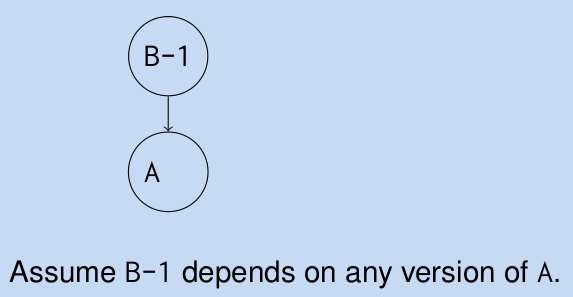
\includegraphics[width=10cm]{image201110/cabal-1.png}
  \end{center}
  \label{fig:cabal-1}\caption{Hackage DB$B>e$G(BB-1$B%Q%C%1!<%8$,(BA$B$K0MB8$7$F$$$k>l9g(B}
\end{figure}

$B$^$:>e?^$N$h$&$K(BHackage DB$B$G(BB-1$B%Q%C%1!<%8$,(BA$B%Q%C%1!<%8$K0MB8$7$F$$$k>l9g$r(B
$B9M$($^$9!#$3$N;~(BB-1$B$O(BA$B$N%P!<%8%g%s$K$D$$$FFC$K;XDj$7$F$$$J$$$H$7$^$9!#(B

\begin{figure}[ht]
  \begin{center}
    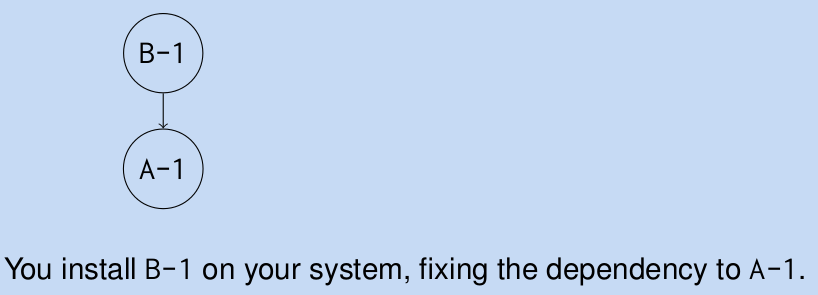
\includegraphics[width=10cm]{image201110/cabal-2.png}
  \end{center}
  \label{fig:cabal-2}\caption{B-1$B$H(BA-1$B$r%$%s%9%H!<%k(B}
\end{figure}

$B$3$N$h$&$J(BHackage DB$B$+$i(BB-1$B$r%$%s%9%H!<%k$9$k$H(BA$B%Q%C%1!<%8$N:G?7%P!<%8%g%s(B
$B$G$"$k(BA-1$B$b0l=o$K%$%s%9%H!<%k$5$l$^$9!#(B

\begin{figure}[ht]
  \begin{center}
    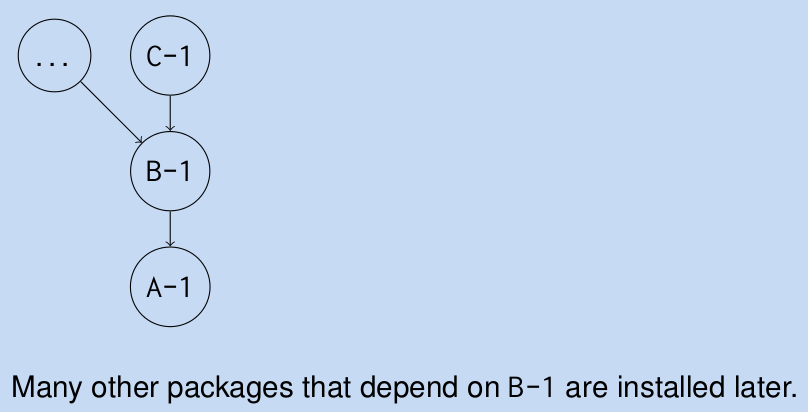
\includegraphics[width=10cm]{image201110/cabal-3.png}
  \end{center}
  \label{fig:cabal-3}\caption{$B$=$7$F$5$i$K(BB-1$B$K0MB8$7$?(BHackage$B72$r%$%s%9%H!<%k(B}
\end{figure}

$B$=$&$7$F!"$3$N$h$&$J4D6-$K$5$i$K(BC-1$B$r4^$`(BB-1$B0MB8$7$?(BHackage$B72$r%$%s%9%H!<%k(B
$B$7$^$9!#$3$3$G!"(BB$B$K0MB8$7$F$$$k(BC-1$B$O%m!<%+%k$G$O(BB-1$B$KI3$E$1$i$l$F$$$^$9!#(B

\begin{figure}[ht]
  \begin{center}
    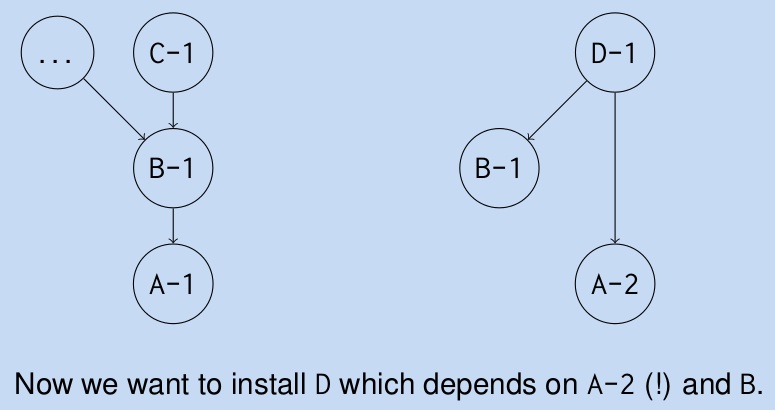
\includegraphics[width=10cm]{image201110/cabal-4.png}
  \end{center}
  \label{fig:cabal-4}\caption{A-2$B$K0MB8$7$F$$$k(BD-1$B$r%$%s%9%H!<%k$7$h$&$H;n$_$k(B}
\end{figure}

$B$3$3$G(BHackage DB$B$+$i(BD-1$B$r%$%s%9%H!<%k$7$F$_$^$7$g$&!#(B
D-1$B$O(BHackage DB$B>e(B($B>e?^1&(B)$B$G$O(BA-2$B$H(BB-1$B$K%P!<%8%g%s;XDj$G0MB8$7$F$$$^$9!#(B
$B%m!<%+%k$K$O(BA-1$B$H(BB-1$B$,%$%s%9%H!<%k$5$l$F$$$^$9!#(B

\begin{figure}[ht]
  \begin{center}
    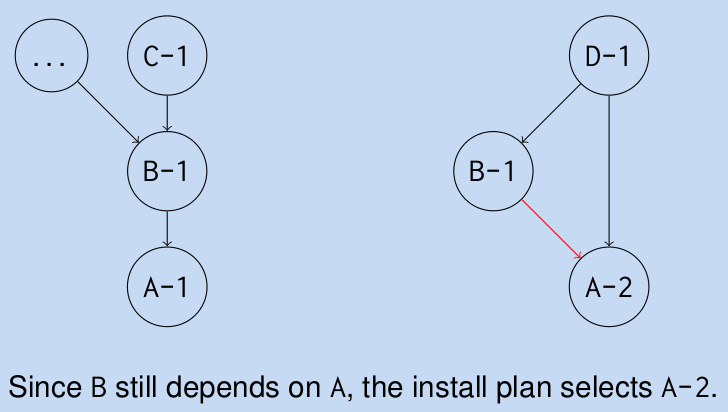
\includegraphics[width=10cm]{image201110/cabal-5.png}
  \end{center}
  \label{fig:cabal-5}\caption{cabal$B$O(BD-1$B$r%$%s%9%H!<%k$K$"$?$C$F(BA-2$B$b%$%s%9%H!<%k$7$h$&$H$9$k(B}
\end{figure}

$B$3$N$^$^%m!<%+%k$K%$%s%9%H!<%k$5$l$F$$$k(BA-1$B$H(BB-1$B$rL5JQ99$G(BD-1$B$r%$%s%9%H!<%k(B
$B$9$k$3$H$O$G$-$^$;$s!#$=$3$G!"(Bcabal$B$O%$%s%9%H!<%k7W2h$r$?$F!"(B
A-1$B$N$+$o$j$K(BA-2$B$r%$%s%9%H!<%k$7$h$&$H$7$^$9!#(B

\begin{figure}[ht]
  \begin{center}
    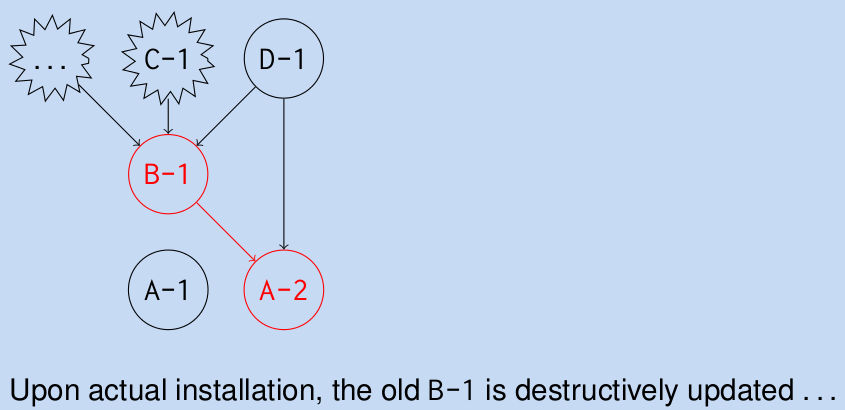
\includegraphics[width=10cm]{image201110/cabal-6.png}
  \end{center}
  \label{fig:cabal-6}\caption{D-1$B$O@5>o$K%$%s%9%H!<%k$5$l$?$,!"(BB-1$B$K0MB8$7$F$$$?(BHackage$B72$O0MB8$,2u$l$F$7$^$&(B}
\end{figure}

A-2,B-1,D-1$B$K$D$$$F(Bcabal$B$O%$%s%9%H!<%k(B/$B99?7$r40N;$7$^$7$?!#(B
$B$7$+$7!"(BB-1$B$K0MB8$7$F$$$?(BHackage$B$K$D$$$F$O:F%3%s%Q%$%k$O9T$J$$$^$;$s!#(B
$BEvA3(BB-1$B$K0MB8$7$F$$$?(BHackage$B$O0MB8$,2u$l$?$^$^J|CV$5$l$F$7$^$&$3$H$K$J$j$^$9!#(B

$B$3$NLdBj$O0MB82r7h$9$k:]$N%$%s%9%H!<%k7W2h$N:]$K%P%C%/%H%i%C%/$,9T$J$o$l$J$$(B
$B$?$a$G$9!#(BB-1$B$r:F%$%s%9%H!<%k$9$k$N$G$"$l$P!"$=$l$K0MB8$7$?(BHackage(C-1$B$J$I(B)
$B$b:F%$%s%9%H!<%k$9$Y$-$@$C$?$N$G$9!#(B
$B$b$A$m$s(BHaskell$B%3%_%e%K%F%#$G$O$3$NLdBj$rG'<1$7$F$*$j!"$=$N2r7h$N$?$a$K(B
$B?7$7$$%=%k%P$r<BAu$7$F$$$^$9!#(B
\footnote{\url{http://darcs.haskell.org/cabal-branches/cabal-modular-solver}}
$B6a$$>-Mh$KK\2H(Bcabal$B$K<h$j9~$^$l$k$3$H$G$7$g$&!#(B

\subsubsection{Hackage$B$,0MB8$9$k4D6-$K$D$$$F(Bcabal$B%3%^%s%I$OLLE]$r$_$F$/$l$J$$(B}

cairo
\footnote{\url{http://hackage.haskell.org/package/cairo}}
$B$N$h$&$K(BC$B8@8l$K0MB8$9$k(BHackage$B$K$D$$$F$O(Bcabal$B%3%^%s%I$OLLE]$r8+$F$/$l$^$;$s!#(B
Debian$B%Q%C%1!<%8(Blibcairo2-dev$B$,F~$C$F$$$J$$4D6-$G(B
cairo Hackage$B$r(Bcabal$B%3%^%s%I$r;H$C$F%$%s%9%H!<%k$7$h$&$H$7$F$b!"(B
($BEvA3(B)$B%3%s%Q%$%k%(%i!<$K$h$C$F%$%s%9%H!<%k$K<:GT$7$^$9!#(B

$B$=$b$=$b(BDebian$B$G$O(BHaskell$B0J30$NItJ,$N%Q%C%1!<%8$O(BDebian$B%Q%C%1!<%8(B(deb)$B$K$h$C$F4IM}$5$l$F$$$^$9!#(B
cabal$B%3%^%s%I$O(BOS$B$K0MB8$7$F$$$J$$$N$G!"(B($BEvA3(B)apt-get$B$r8F$S=P$9$o$1$K$b$$$-$^$;$s!#(B
\footnote{\url{http://packages.debian.org/ja/sid/auto-apt}
$B$r;H$C$F(Bcabal$B%3%^%s%I<B9T$NN"$G(BDebian$B%Q%C%1!<%8$r<+F0%$%s%9%H!<%k$9$k<j$O$"$k$+$b$7$l$^$;$s$M(B ;-)}

\subsubsection{Hackage$B72A4$F$r:G?7%P!<%8%g%s$G%$%s%9%H!<%k$G$-$J$$$+$b$7$l$J$$(B}

yesod \footnote{\url{http://hackage.haskell.org/package/yesod}}
,hakyll \footnote{\url{http://hackage.haskell.org/package/hakyll}}
,hamlet \footnote{\url{http://hackage.haskell.org/package/hamlet}}
$B$N(B3$B$D$N(BHackage$B$rNc$K@bL@$7$^$9!#(B
$B$3$NLdBj$O(Byesod-0.9.2, hakyll-3.2.0.8, hamlet-0.10.2$B$N%P!<%8%g%s4V$G@8$8$F$$$^$7$?!#(B($B8=:_$O2r>C$5$l$F$$$^$9(B)

$B$^$:$=$l$>$l$N(BHackage$B$K$D$$$F0MB8$r8+$F$_$^$7$g$&!#(B

\begin{commandline}
$ cabal info yesod-0.9.2
* yesod-0.9.2            (program and library)
--snip--
    Dependencies:  yesod-core >=0.9.1.1 && <0.10, yesod-auth ==0.7.*,
--snip--
                   hamlet ==0.10.*, shakespeare-js ==0.10.*,
--snip--
$ cabal info hakyll-3.2.0.8
* hakyll-3.2.0.8           (library)
--snip--
    Dependencies:  base ==4.*, binary >=0.5 && <1.0, blaze-html >=0.4 && <0.6,
--snip--
                   filepath >=1.0 && <2.0, hamlet >=0.7 && <0.9,
\end{commandline}

$B$"$l!)(Byesod-0.9.2$B$O(Bhamlet-0.10.*$B$K0MB8$7$F$$$k$N$K(Bhakyll-3.2.0.8$B$O(B
hamlet-0.7.*$B$b$7$/$O(Bhamlet-0.8.*$B$K0MB8$7$F$$$^$9!#(B
$B3N$+$KI=LL>eLdBj$O$"$j$^$;$s!#$3$N>uBV$G$b(Byesod$B$H(Bhakyll$B$NN>J}$r%$%s%9%H!<%k(B
$B$9$k$3$H$O$G$-$^$9!#$7$+$7$b$7(Bhakyll$B$H(Byesod$BN>J}$N%i%$%V%i%j$r;H$$$?$$%W%m%0%i%`(B
$B$r:n$j$?$/$J$C$?>l9g$K$O$I$&$7$?$iNI$$$N$G$7$g$&!)(B
hakyll$B$O%m!<%+%k$G(BWeb$B%5!<%P$r5/F0$7$F%W%l%S%e!<$9$k5!G=$r;}$C$F$$$^$9!#(B
$B$?$^$?$^(Bhakyll$B$O$3$N(BWeb$B%5!<%P$N%(%s%8%s$H$7$F(Bsnap
\footnote{\url{http://hackage.haskell.org/package/snap}}
$B$r;H$C$F$$$?$+$iNI$+$C$?$b$N$N(Byesod$B$r;H$C$F$$$?$i!"8E$$(Byesod$B$N5!G=(B
$B$7$+;H$($J$$$H$3$m$G$9!#(B

$B$I$&$7$F$3$s$J>uBV$G(BHackage$B$,J|CV$5$l$F$$$?$N$G$7$g$&!)(B
$B$d$k5$$,$J$$$N$G$7$g$&$+!)$$$($$$($=$s$J$3$H$O$"$j$^$;$s!#(B
$B:#EY$O(Bhamlet$B$K$D$$$FD4$Y$F$_$^$7$g$&!#(B

\begin{commandline}
# hamlet-0.8.2.1$B$N(BModule$B%j%9%H(B
Text
  Text.Cassius
  Text.Coffee
  Text.Hamlet
    Text.Hamlet.NonPoly
    Text.Hamlet.RT
  Text.Julius
  Text.Lucius
  Text.Romeo
  Text.Shakespeare

# hamlet-0.9.0$B$N(BModule$B%j%9%H(B
Text
  Text.Cassius
  Text.Coffee
  Text.Hamlet
  Text.Julius
  Text.Lucius
  Text.Romeo
  Text.Shakespeare
\end{commandline}

$B$"$l!)(BAPI$B$KJQ99$,$"$k$h$&$G$9!#$3$3$GCmL\$7$?$$$N$O(BText.Hamlet.RT$B%b%8%e!<%k$,(B
$B>CLG$7$F$$$k$3$H$G$9!#(B
$B7y$JM=46$,$7$^$9!#(Bhakyll$B$N%=!<%9%3!<%I(B
\footnote{\url{https://github.com/jaspervdj/hakyll/blob/master/src/Hakyll/Web/Template/Read/Hamlet.hs}}
$B$r8+$F$_$^$7$g$&!#(B

\begin{commandline}
-- | Read templates in the hamlet format
--
{-# LANGUAGE MultiParamTypeClasses #-}
module Hakyll.Web.Template.Read.Hamlet
    ( readHamletTemplate
    , readHamletTemplateWith
    ) where

import Text.Hamlet (HamletSettings, defaultHamletSettings)
import Text.Hamlet.RT

import Hakyll.Web.Template.Internal
--snip--
\end{commandline}

$B$"!<(Bhakyll$B$N%3%s%Q%$%k$K$O(BText.Hamlet.RT$B%b%8%e!<%k$,I,?\$J$s$G$9$M!#(B
$B$3$l$G$O?7$7$$(Bhamlet$B$r;H$&$3$H$,$G$-$J$$Lu$G$9!#(B

Hackage$B:n<T$,<+M3$K0MB8(BHackage$B$N%P!<%8%g%s$rA*Br2DG=$G$"$k0J>e!"(B
$B$3$N$h$&$J(BHackage$B72A4BN$NIT@09g$OHr$1$i$l$^$;$s!#(B

\subsection{Hackage$B$r(BDebian$B%Q%C%1!<%82=$9$k(B}

cabal$B$r;H$C$F(BDebian$B%Q%C%1!<%8$HF1Ey$N%l%Y%k$G(B
$B%Q%C%1!<%84IM}$r$9$k$N$O8=>u$G$OFq$7$$$3$H$,$o$+$j$^$7$?!#(B
$B$=$l$K(Bapt-get$B$G%i%$%V%i%j4D6-$,@0$&$N$O(BDebian$B%f!<%6$H$7$F$&$l$7$$$G$9$h$M!#(B
$B$=$3$G!"<+J,$NNI$/;H$&(BHackage$B$O(BDebian$B%Q%C%1!<%82=$7$F(BDebian$BK\BN$K(B
$BEPO?$7$F$7$^$&$N$O$$$+$,$G$7$g$&$+!#(B
$B<B$O(BHackage$B$r(BDebian$B%Q%C%1!<%82=$9$k$N$O$9$4$/4JC1$G$9!#(B
cabal-debian \footnote{\url{http://hackage.haskell.org/package/debian}}
$B$H$$$&$^$s$^$NL>A0$N%3%^%s%I$,$"$j$^$9!#(B
$B$5$C$=$/$d$C$F$_$^$7$g$&(B!

$BNcBj$H$7$F(BHCWiid
\footnote{Wii$B%j%b%3%s$+$i%$%Y%s%H$r=&$&$?$a$N%i%$%V%i%j(B
  \url{http://hackage.haskell.org/package/hcwiid}}
$B$r(BDebian$B%Q%C%1!<%82=$7$F$_$^$9!#(B
$B$^$:(BHackage$B$N(BDebian$B%Q%C%1!<%82=$KI,MW$J(Bhaskell-debian-utils,
haskell-devscripts$B$r(Bapt-get install$B$7$^$7$g$&!#(B

\begin{commandline}
$ sudo apt-get install haskell-debian-utils haskell-devscripts
$ rehash
\end{commandline}

hackage$B$r%@%&%s%m!<%I$7$F2rE`$7$?$i!"%G%#%l%/%H%j$K0\F0$7$F$*$b$`$m$K(Bcabal-debian$B%3%^%s%I$r;H$$$^$9!#(B

\begin{commandline}
$ wget http://hackage.haskell.org/packages/archive/hcwiid/0.0.1/hcwiid-0.0.1.tar.gz
$ tar xfz hcwiid-0.0.1.tar.gz
$ cd hcwiid-0.0.1/
$ cabal-debian --debianize --ghc --maintainer="Kiwamu Okabe <kiwamu@debian.or.jp>"
$ ls debian
changelog  compat  control  copyright  rules*
$ debuild -rfakeroot -us -uc
--snip--
 dpkg-genchanges  >../haskell-hcwiid_0.0.1-1~hackage1_amd64.changes
dpkg-genchanges: including full source code in upload
 dpkg-source --after-build hcwiid-0.0.1
dpkg-buildpackage: full upload; Debian-native package (full source is included)
Now running lintian...
W: haskell-hcwiid source: native-package-with-dash-version
W: haskell-hcwiid source: out-of-date-standards-version 3.9.1 (current is 3.9.2)
E: libghc-hcwiid-dev: copyright-file-contains-full-gpl-license
E: libghc-hcwiid-dev: copyright-should-refer-to-common-license-file-for-lgpl
E: libghc-hcwiid-dev: description-contains-tabs
E: libghc-hcwiid-prof: copyright-file-contains-full-gpl-license
E: libghc-hcwiid-prof: copyright-should-refer-to-common-license-file-for-lgpl
E: libghc-hcwiid-prof: description-contains-tabs
E: libghc-hcwiid-doc: copyright-file-contains-full-gpl-license
E: libghc-hcwiid-doc: copyright-should-refer-to-common-license-file-for-lgpl
E: libghc-hcwiid-doc: description-contains-tabs
Finished running lintian.
$ ls ../*hcwiid*deb
../libghc-hcwiid-dev_0.0.1-1~hackage1_amd64.deb
../libghc-hcwiid-doc_0.0.1-1~hackage1_all.deb
../libghc-hcwiid-prof_0.0.1-1~hackage1_amd64.deb
\end{commandline}

$B$J$s$+$"$C$5$j(BDebian$B%Q%C%1!<%8$,$G$-$A$c$$$^$7$?!#(B
lintian$B$,$J$s$+8@$C$F$^$9$,!"(B
$B$"$^$j?<9o$J$b$N$G$O$J$$$N$G$H$j$"$($:%$%s%9%H!<%k$7$F$_$^$7$g$&!#(B

\begin{commandline}
$ sudo dpkg -i ../libghc-hcwiid-dev_0.0.1-1\~hackage1_amd64.deb ../libghc-hcwiid-doc_0.0.1-1\~hackage1_all.deb ../libghc-hcwiid-prof_0.0.1-1\~hackage1_amd64.deb
$ cd ~/
$ rm -rf .ghc .cabal
# $B$3$l$G(Bcabal$B$G%$%s%9%H!<%k$7$?%Q%C%1!<%8$O0l@Z;H$C$F$$$J$$$O$:$G$9(B
$ ghc-pkg list|grep hcwiid
    hcwiid-0.0.1
# Hackage$B$O%$%s%9%H!<%k:Q$_$N$h$&$G$9(B
# hcwiid$B%i%$%V%i%j$r;H$C$F$_$^$7$g$&(B
$ vi Test.hs
module Main where

import Prelude
import Control.Monad
import System.CWiid
import System.Posix.Unistd

main :: IO ()
main = do
  putStrLn "Put Wiimote in discoverable mode now (press 1+2)..."
  (Just wm) <- cwiidOpen
  putStrLn "found!"
  _ <- cwiidSetLed wm
  _ <- cwiidSetRptMode wm
  _ <- forever $ do _ <- usleep 300000
                    cwiidGetBtnState wm >>= print
  return () -- not reach
$ ghc --make Test.hs
[1 of 1] Compiling Main             ( Test.hs, Test.o )
Linking Test ...
$ ./Test
Put Wiimote in discoverable mode now (press 1+2)...
\end{commandline}

$B$J$s$F4JC1$J$s$G$7$g$&(B!$B4JC1$J(BHackage$B$J$i(Bcabal-debian$B%3%^%s%I$r;H$($P(B
Debian$B%Q%C%1!<%82=$,40N;$7$F$7$^$&$h$&$G$9!#(B
$B$7$+$b2<5-(B3$B$D$N%i%$%V%i%j$KJ,3d$7$F$/$l$F$$$^$9!#$d$C$?(B!

\begin{itemize}
 \item libghc-HOGE-dev  - $BDL>o;HMQ$9$k%i%$%V%i%j(B
 \item libghc-HOGE-doc  - Haddock$B$G@8@.$5$l$?(BAPI$B%I%-%e%a%s%H(B
 \item libghc-HOGE-prof - $B%W%m%U%!%$%iBP1~%i%$%V%i%j(B
\end{itemize}

\subsection{haskell-debian-utils$B$N$7$/$_(B}

cabal-debian$B$G$N(BDebian$B%Q%C%1!<%82=$O$I$N$h$&$J$7$/$_$J$N$G$7$g$&$+!#(B
$B$5$-$[$I:n$C$?(Bhcwiid$B%Q%C%1!<%8$N(Bdebian/rules$B%U%!%$%k$r8+$F$_$^$7$g$&!#(B

\begin{commandline}
#!/usr/bin/make -f
include /usr/share/cdbs/1/rules/debhelper.mk
include /usr/share/cdbs/1/class/hlibrary.mk

# How to install an extra file into the documentation package
#binary-fixup/libghc-hcwiid-doc::
#       echo "Some informative text" > debian/libghc-hcwiid-doc/usr/share/doc/libghc-hcwiid-doc/AnExtraDocFile
\end{commandline}

$B$J$s$H$$$&$3$H$G$7$g$&!#FbMF$,$J$$$G$9!#!#!#(B
$B$3$l$O(Bhlibrary.mk$B%U%!%$%k$KHkL)$,$"$k$KAj0c$"$j$^$;$s!#(B
$BA4It$rFI$^$:$K$^$:$O(Blibghc-HOGE-dev$B$N(Bbuild$B%?!<%2%C%H$H$=$N6aJU$r(Bhlibrary.mk
$B$+$iH4$-=P$7$F$_$^$7$g$&!#(B

\begin{commandline}
DEB_SETUP_BIN_NAME ?= debian/hlibrary.setup
BUILD_GHC := $(DEB_SETUP_BIN_NAME) build

$(DEB_SETUP_BIN_NAME):
        if test ! -e Setup.lhs -a ! -e Setup.hs; then echo "No setup script found!"; exit 1; fi
        for setup in Setup.lhs Setup.hs; do if test -e $$setup; then ghc --make $$setup -o $(DEB_SETUP_BIN_NAME); \
          exit 0; fi; done

build/libghc-$(CABAL_PACKAGE)-prof build/libghc-$(CABAL_PACKAGE)-dev:: build-ghc-stamp

build-ghc-stamp: dist-ghc
        $(BUILD_GHC) --builddir=dist-ghc
        touch build-ghc-stamp
\end{commandline}

$B$J$k$[$I!#(Blibghc-HOGE-dev$B$r(Bbuild$B$7$h$&$H$9$k$H!"(B
$B$^$:(BSetup.lhs$B$b$7$/$O(BSetup.hs$B$r(Bghc$B$r;H$C$F%3%s%Q%$%k$7$F(Bdebian/hlibrary.setup
$B%3%^%s%I$r:n@.$9$k$h$&$G$9!#(B
$B$=$&$7$F:n$C$?(Bdebian/hlibrary.setup$B%3%^%s%I$r;H$C$F(B
"debian/hlibrary.setup build --builddir=dist-ghc"
$B$N$h$&$K$7$F(Bdist-ghc$B%G%#%l%/%H%j>e$G(BHackage$B$r%3%s%Q%$%k$9$k$s$G$9$M!#(B

$B$A$g$C$HC&@~$7$^$9$,!"(B
$B$3$N%S%k%I%W%m%;%9$O(Bcabal$B$,IaCJ$d$C$F$$$k$3$H$HA4$/F1$8$G$9!#(B
cabal$B$O%$%s%9%H!<%kBP>]$N(BHackage$B$r<hF@(B/$BE83+$7$?$i!"$^$:$3$N(BSetup.hs$B$r(B
ghc$B$G%3%s%Q%$%k$7$F!"$=$N%3%s%Q%$%k$7$?7k2L$G$-$?<B9T%P%$%J%j$r(B
$BK\Ev$N%S%k%@(B/$B%$%s%9%H!<%i$H$7$F;H$$$^$9!#(B
$BIaCJ;H$C$F$$$k(B/usr/bin/cabal$B%3%^%s%I$O(B"cabal-install"$B$H8F$P$l$F$$$^$9!#(B
$B$=$7$F!"(BSetup.hs$B$r=q$/$?$a$KI,MW$J%i%$%V%i%j$r(B"Cabal"$B$H8F$S$^$9!#(B
$B$d$d$3$7$$$G$9$M!#!#!#(B

$B$G$O(Blibghc-HOGE-dev$B$N(Binstall$B$O$I$&$J$C$F$$$k$N$G$7$g$&$+!)(B

\begin{commandline}
debian/tmp-inst-ghc: $(DEB_SETUP_BIN_NAME) dist-ghc
	$(DEB_SETUP_BIN_NAME) copy --builddir=dist-ghc --destdir=debian/tmp-inst-ghc

install/libghc-$(CABAL_PACKAGE)-dev:: debian/tmp-inst-ghc debian/extra-depends
	cd debian/tmp-inst-ghc ; find usr/lib/haskell-packages/ghc/lib/ \
		\( ! -name "*_p.a" ! -name "*.p_hi" \) \
		-exec install -Dm 644 '{}' ../$(notdir $@)/'{}' ';'
	pkg_config=`$(DEB_SETUP_BIN_NAME) register --builddir=dist-ghc --gen-pkg-config | sed -r 's,.*: ,,'`; \
		$(if $(HASKELL_HIDE_PACKAGES),sed -i 's/^exposed: True$$/exposed: False/' $$pkg_config;) \
		install -Dm 644 $$pkg_config debian/$(notdir $@)/var/lib/ghc/package.conf.d/$$pkg_config; \
		rm -f $$pkg_config
	if [ 'z$(DEB_GHC_EXTRA_PACKAGES)' != 'z' ] ; then \
		echo '$(DEB_GHC_EXTRA_PACKAGES)' > \
                debian/$(notdir $@)/usr/lib/haskell-packages/ghc/lib/$(CABAL_PACKAGE)-$(CABAL_VERSION)/extra-packages ; \
	fi
	dh_haskell_provides -p$(notdir $@)
	dh_haskell_depends -p$(notdir $@)
	dh_haskell_shlibdeps -p$(notdir $@)
\end{commandline}

$B$A$g$C$H$o$+$j$K$/$$$G$9$,!"%Q%C%1!<%82=$N8eH>$O(BDebian$BN.57$N>\:Y$J$N$G(B
$BF'$_$3$^$:$K2r<a$9$k$H!"(B
$B$^$:(Blibghc-HOGE-dev$B$r(Binstall$B$7$h$&$H$9$k$H!"(Bdebian/tmp-inst-ghc$B%?!<%2%C%H(B
$B$,8F$S=P$5$l$F(B
"debian/hlibrary.setup copy --builddir=dist-ghc --destdir=debian/tmp-inst-ghc"
$B$N$h$&$J%3%^%s%I$,<B9T$5$l$F!"(Bdist-ghc$B$G%3%s%Q%$%k$7$?FbMF$,(B
debian/tmp-inst-ghc$B0J2<$K%$%s%9%H!<%k$5$l$^$9!#(B
$B$"$H$O!"(BDebian$B$NN.57$K$N$C$H$C$F(Bdebian/tmp-inst-ghc$B0J2<$N%U%!%$%k72$r(B
$B%Q%C%1!<%82=$9$k$@$1$G$9!#(B
$B%Q%C%1!<%82=BP>]$N(BHackage$B$,0MB8$7$F$$$k(BHackage$B$b(B
dh\_haskell\_shlibdeps$B$G$A$c$s$H8!=P$7$F$/$l$k$_$?$$$G$9!#(B :)

\subsection{$B:n$C$?%Q%C%1!<%8$r(BDebian$B$KEPO?$9$k$K$O(B}

$B$;$C$+$/:n$C$?(BHackage$B$G$9!#<+J,$@$1$G;H$C$F$$$k$N$O$b$C$?$$$J$$$G$9!#(B
Debian$BK\2H$KEPO?$7$F3'$K;H$C$F$b$i$$$^$7$g$&(B!
Debian$BK\2H$KEPO?$7$F$*$1$P$a$0$j$a$0$C$F(BUbuntu$B$K$bEPO?$5$l$k$+$b$7$l$^$;$s$h!)(B

Debian$B%Q%C%1!<%82=$5$l$?(BHackage$B72$O(Bdarcs$B$G%P!<%8%g%s4IM}$5$l$F$$$^$9!#(B

xxxxx pkg-haskell$B$d$i(Bdarcs$B$NOC$d$i(B

%-------------------------------------------------------------------------------
\dancersection{$B7n4)(B debhelper}{$B4d>>(B $B?.MN(B}
%-------------------------------------------------------------------------------
\index{debhelper}

\subsection{debhelper $B$H$O2?$+!)(B}

Debian $B%Q%C%1!<%8$OMM!9$J=hM}$,9T$o$l$F$*$j!"$3$l$i$r$R$H$D$E$D=q$$$F$$$/$HKDBg$JNL$K$J$j$^$9!#(B
$B$^$?!"%3!<%I$NNL$,B?$/$J$k$H%P%0$bB?$/$J$j!"LdBj$,5/$-$?$H$-$K=$@5$9$k$N$OBgJQ$G$9!#(B
$B$3$l$i$N=hM}$r5!G=Kh$K$^$H$a!";H$$$d$9$/$7$?5!G=$rDs6!$7$F$$$k%Q%C%1!<%8$H$7$F(B debhelper $B$,$"$j$^$9!#(B
$BB>$K$bF1MM$N%D!<%k$,$"$j$^$9$,!"0lHV;H$o$l$F$$$k$N$,$3$N(B debhelper $B$G$9!#(B
Debian $B%Q%C%1!<%8$r%a%s%F%J%s%9$7$F$$$k?M$K$H$C$F$J$/$F$O$J$i$J$$B8:_$H$J$C$F$$$^$9!#(B
debhelper $B$O(B Debian $B3+H/<T$N(B Joey Hess $B;a(B\footnote{Wiki$B%(%s%8%s$N(Bikiwiki, $B%G%#%9%H%j%S%e!<%7%g%s$N%Q%C%1!<%8JQ49%D!<%k$G$"$k(Balien $B$N3+H/<T$H$7$FM-L>!#(B}
$B$K$h$C$F3+H/(B/$B%a%s%F%J%s%9$5$l!":G?7$N%P!<%8%g%s$O(B 8.9.8 $B$H$J$C$F$$$^$9!#(B

\subsection{$B7n4)(B debhelper}
$B@h$K$b@bL@$7$?$h$&$K!"(Bdebhelper $B$O(BDebian$B%Q%C%1!<%8$r%a%s%F%J%s%9$9$k?M$K$H$C$F$J$/$F$O$J$i$J$$%D!<%k$N0l$D$G$9!#(B
Debian$B%Q%C%1!<%8$r%a%s%F%J%s%9$7$F$$$k?M$O(Bdebhelper$B$,$I$N$h$&$J5!G=$rDs6!$7$F!"$I$N$h$&$K$D$+$C$F$$$1$P$$$$$N$+(B
$BM}2r$7$F$*$/I,MW$,$"$j$^$9!#$H$$$C$F$b(Bdebhelper $B$G$O(B59$B8D$N%3%^%s%I!J(Bdh\_$B$G;O$^$k%3%^%s%I!K$,Ds6!$5$l$F$*$j!"(B
$BA4ItM}2r$9$k$N$OFq$7$$$G$7$g$&!#$^$?!"(Bdebhelper $B$K<}O?$5$l$F$$$J$$(B debhelper $B%5%]!<%H%D!<%k$r4^$a$k$H(B100$B8D$[$I$K$J$j$^$9!#(B
$BF|:"(BDebian$B$N3+H/$r9T$J$C$F$$$k?M$G$b!V$"$"!"$3$s$J5!G=$,$"$k$N$@!W$H;W$&$3$H$,$"$k$0$i$$$G$9!#(B
$B$3$N$h$&$J$3$H$b$"$j!"$3$N7n4)(B debhelper $B$G$O$3$l$i$N%3%^%s%I$NF0$-$H;H$$J}$rKh7n?t8D$E$D>R2p$7!"(BDebian$BJY6/2q;22C<T$G%Q%C(B
$B%1!<%8:n@.$NM}2r$r?<$a$k$H$$$&$b$N$G$9!#A4$FM}2r$7$?:"$K$O3'!"(BDebian$B%Q%C%1!<%8%a%s%F%J$K$J$C$F$$$k$+$b$7$l$^$;$s!#(B
$B%R%c%C%O!<!*(B

\subsubsection{$B7n4)(B debhelper $B0-Kb$N%k!<%k(B}
$BKh7n?t8D$E$D>R2p$9$k$H$$$C$F$b!"F1$8?M$,Kh2s65$($F$$$F$OLLGr$/$"$j$^$;$s!J8D?ME*$K!K!#(B
Debian{\bf $BJY6/2q(B}$B$J$N$G!"Kh7n;}$A2s$j$G3F(B debhelper $B%3%^%s%I$r>R2p$9$k$H$$$&J}K!$r<h$j$^$9!#(B
$B0J2<$,;d$,>!<j$K7h$a$?$R$I$$%k!<%k$G$9!#(B

\begin{itemize}
\item $B0l?M0l8D0J>e$N(B debhelper $B%3%^%s%I$N@bL@$r$9$k!#(B
\item $BEv7n$NH/I=<T$,<!$KH/I=$5$;$k?M$r7h$a$k$3$H$,$G$-$k!#(B
\item $B$?$@$7!"<+J,$GN)8uJd$9$k>l9g$O$=$N8B$j$G$O$J$$!#(B
\item $BB3$1$FH/I=$G$-$J$$!#:GBg(B2$B2s6u$1$k$3$H!#(B
\item $B0lHV:G=i$KH/I=<T?M$,%k!<%k$r7h$a$k$3$H$,$G$-$k!#(B
\end{itemize}

$BAa$/H/I=$9$k$HHf3SE*4JC1$J$b$N$H$+!"<+J,$,JY6/$7$?$$$b$N$+$iH/I=$G$-$k$+$b$7$l$^$;$s!#(B

\subsection{$B:#7n$N%3%^%s%I(B}

dh\_scrollkeeper
dh\_shlibdeps
dh\_install


\subsection{$B<!$NH/I=<T(B}
$B<!$NH/I=<T$O(B $BA0ED$5$s$G$9!#(B
$B4hD%$C$F$/$@$5$$!#(B


\printindex

\cleartooddpage

\vspace*{15cm}
\hrule
\vspace{2mm}

\includegraphics[width=2cm]{image200502/openlogo-nd.eps}
\noindent \Large \bf Debian $BJY6/2q;qNA(B\\
\noindent \normalfont \debmtgyear{}$BG/(B\debmtgmonth{}$B7n(B\debmtgdate{}$BF|(B \hspace{5mm}  $B=iHGBh(B1$B:~H/9T(B\\
\noindent \normalfont $BEl5~%(%j%"(B Debian $BJY6/2q(B $B!JJT=8!&0u:~!&H/9T!K(B\\
\hrule

\end{document}
